\documentclass{article}
\usepackage{graphicx}
\usepackage[margin=1.5cm]{geometry}
\usepackage{amsmath}
\usepackage{url}

\begin{document}

\title{Midterm 1: College Writing Seminar}
\author{Prof. Jordan C. Hanson}

\maketitle

\textbf{Assigned:} October 9th, 2020 at 9:00 am.  \textbf{Due:} October 12th, 2020 at 9:00 am. Submit all answers in one PDF document, and submit this PDF on Moodle under Week 5.

\section{Week 1: Concise Writing 1}

\begin{enumerate}
\item \textit{Using the delete button.} For the sentences below, re-write them more concisely. \\ \\
\textbf{Create an edited version in your document.}
\begin{enumerate}
\item Knowing the orbits of the stars around the center of the galaxy, scientists use the orbits to calculate the mass of the object at the center of the galaxy.  The object has the mass that is so large the mass has to be of a black hole. \\
\textbf{From the orbits of the stars around the galactic center, the mass of the object they orbit can be shown to be that of a black hole.}
\item Epidemiologists use a parameter called the reproduction parameter, R0, which is the number of new infections
resulting from one new infected person. \\
\textbf{The epidemiological reproduction parameter $R_0$ is the number of new infections resulting from one new infected person.}
\item According to the Newton’s Laws of motion, things that have different masses and different shapes would still
acceleratae downward at the same rate when dropped. \\
\textbf{According to the Newton's Laws of motion, objects of different masses accelerate downward at the same rate due to gravity.}
\end{enumerate}
\item \textit{Creating an outline.} Create an outline of the following set of ideas, such that it describes how to determine optimal tomato growing conditions.  Use the outline to write a well-organized paragraph describing the experiment. Submit \textit{both} the paragraph and the outline.  \\ \\
\textbf{Create a paragraph in your document.} 
\begin{figure}[hb]
\centering
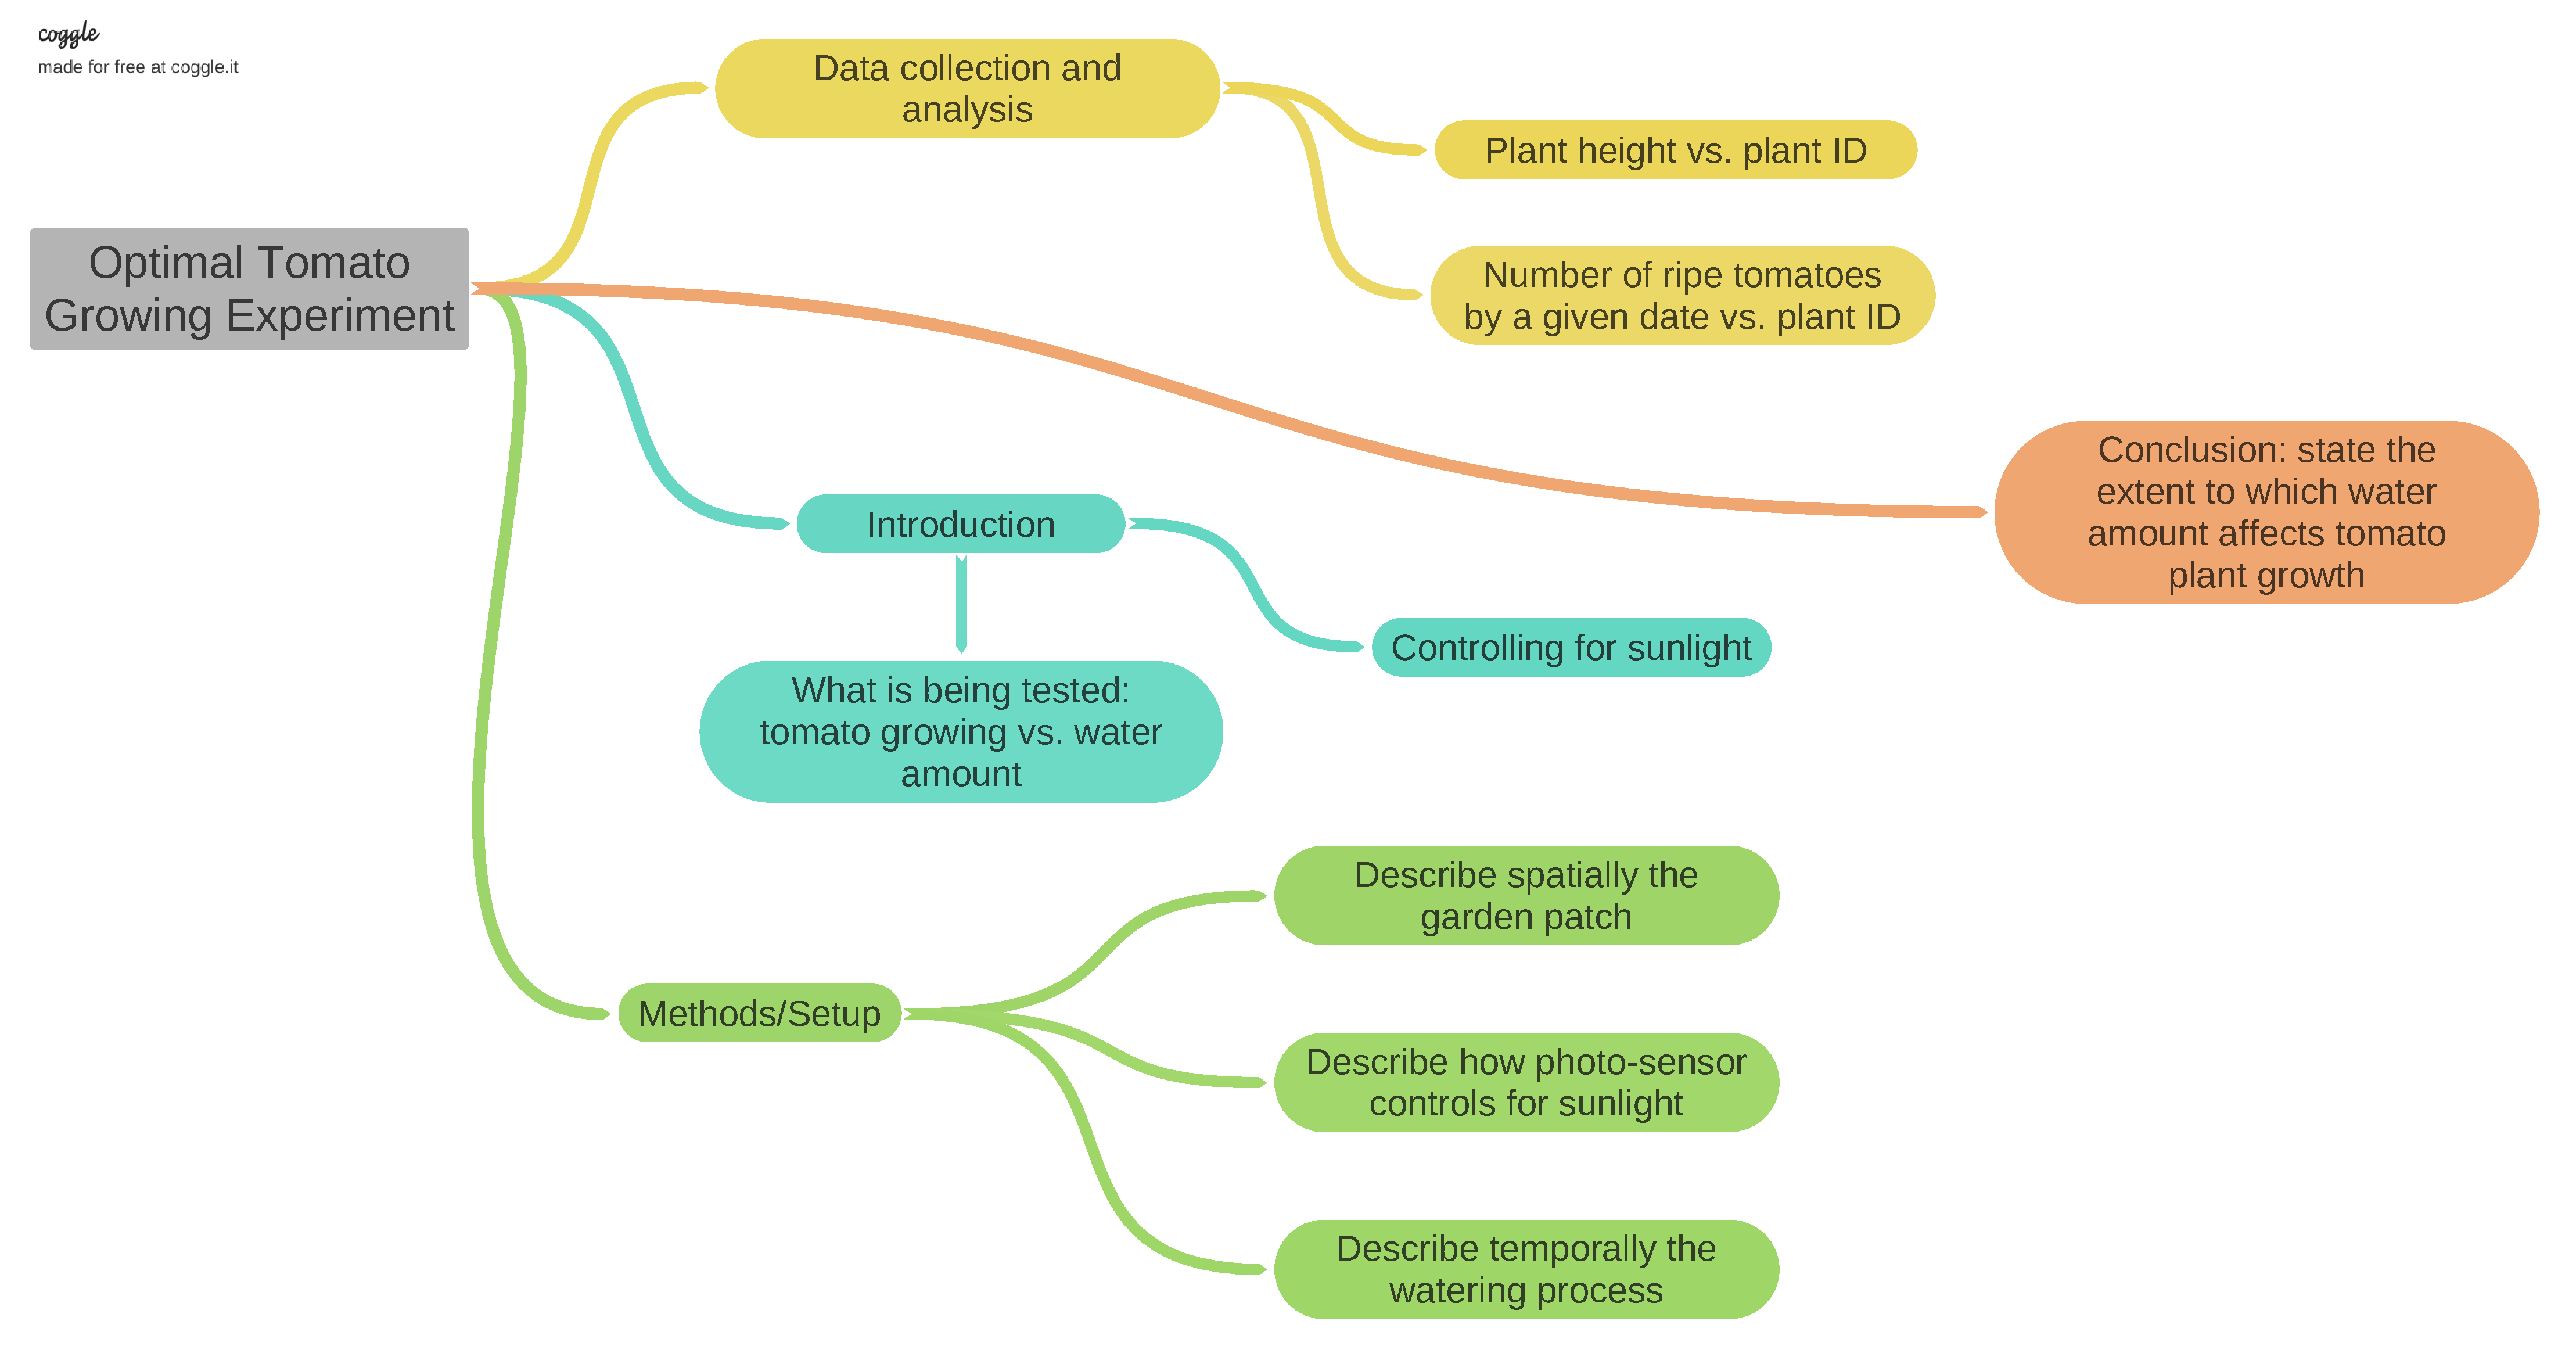
\includegraphics[width=0.65\textwidth]{figures/tomato.pdf}
\caption{\label{fig:tomato} An example of an outline for the tomato growing list.}
\end{figure}
An experiment was conducted to determine the effect of water availability on tomato production while controlling for sunlight.  Ten tomato plants were planted in a row in a patch of garden soil with roughly equal amounts of sunlight in the summer.  A photo-sensor was installed at each site to determine the average solar illumination each day.  Each morning at 10:00 am, all ten tomato plants received water, starting with plant 1 at 100 mL and increasing linearly to 1000 mL by plant 10.  After 60 days of summer, two variables were measured: plant height and the number of ripe tomatos per plant.  Plants that received more water tended to exceed plants that received less water in both variables.
\end{enumerate}

\section{Week 2: Concise Writing 2}

\begin{enumerate}
\item \textit{Hierarchy of detail and outlines}.  Choose from any of the 4 topics from slide 4 of the Week 2 Lecture Notes.  Select 3-4 sources online and use them to create an outline with the appropriate hierachy of details covering the subject.  Submit the outline and a 200 word summary of the subject, written concisely and without ambiguous words or phrasing. Properly cite your sources. \\ \\
\textbf{Add the work to your document.} \\
The IceCube Neutrino Observatory is a neutrino detector formed by a cubic kilometer of ice in Antarctica [2][6]. IceCube could potentially detecto super-novae [6] and other point-sources like blazars [5].  IceCube construction began in 2004, and was completed in 2011 [1]. Construction took place during Antarctic summer when there is 24-hour sunlight [5].  Digital optical modules were lowered into ice boreholes to Cherenkov radiation produced by neutrinos from space [5][7][8]. Properties of the Cherenkov radiation reveal the neutrino energy and direction [5][8]. IceCube’s modules are between 1,450 and 2,450 meters deep where the ice is clearest [3][5]. IceCube is able to distinguish three types of neutrino: electron, muon, and tau [8].  Over the next few years, IceCube will be upgraded to IceCube-Gen2 [1][7]. The purpose of the upgrade is to increase sensitivity to lower-energy neutrinos which it currently cannot detect [7]. The low-energy neutrinos are important for determining neutrino mass properties in addition to energy and direction. Further, increased detector size would improve the angular resolution of IceCube, which would pinpoint more accurately neutrino sources on the sky.  IceCube has opened a new window on the universe, and the field of neutrino astrophysics will continue to grow.
\begin{itemize}
\item [1] University of Wisconsin-Madison. IceCube South Pole Neutrino Observatory. IceCube.wise.edu
\item [2] Nola Taylor Read. IceCube: Unlocking the Secrets of Cosmic Rays. Space.com. 
\item [3] A. Albert et al. Search for High-Energy Neutrinos from Binary Neutron Star Merger GW170817 with Antares, IceCube, and The Pierre Auger Observatory. The Astrophysical Journal Letters, Volume 850, (2), 2017. 
\item [4] The IceCube Collaboration. The IceCube Neutrino Observatory Part IV: Searches for Dark Matter and Exotic Particles. 33rd International Cosmic Ray Conference, Rio de Janeiro 2013 The Astroparticle Physics Conference, 2013. 
\item [5] Stephen Crass. The IceCube Neutrino Detector at the South Pole Hits Paydirt. IEEE Spectrum, 2018. 
\item [6] University of Wisconsin-Madison Department of Astronomy. Neutrinos! Astro.wisc.edu. 
\item [7] Alden L. Coke. The Detection of Neutrinos in IceCube. IceCube Masterclass. 
\item [8] Dawn Williams. Recent Results from IceCube. International Journal of Modern Physics: Conference Series Vol. 46 (2018) 1860048, 2018.
\end{itemize}
\end{enumerate}

\section{Week 3: Technical Description 1}

\begin{enumerate}
\item \textit{Removing ambiguous words.}  In the following sentences, remove or replace ambiguous words. \\ \\
\textbf{Write the new sentences in your own document.} 
\begin{itemize}
\item When born, the baby was fairly heavy and really long. \textbf{When born, the baby was 7 lbs. and 20 inches long.}
\item The baby grew really fast, by the time she was 1 year old, she was a lot longer. \textbf{The baby grew to 30 inches by 1 year.}
\item Radio transmission took a long while between the Earth and the Moon. \textbf{It takes about 3 seconds for a radio transmission to travel from the Earth to the Moon, and back.}
\item A hiker walked the full 60 km trail in 4 days, making her average speed moderate. \textbf{A hiker walked the 60 km trail in 4 days, making her average speed 15 km/day.}
\end{itemize}
\item \textit{Spatial and temporal detail, perspective.}  Recall the exercise we performed in class, in which we wrote our favorite recipe.  In this exercise, explain to the reader from where you are gathering the ingredients, \textit{and} the recipe.  Thus, the result should be a tract of writing that would enable someone to prepare the dish using your kitchen and pantry. Notice how this requires you to pay attention to both time and space. \\ \\
\textbf{Write a paragraph in your own document.} \\
Imagine yourself in a small kitchen with a sink in front of you, and a window above it.  To your right is a pantry above the counter on the wall, and inside on the first shelf is the peanut butter. Collect the peanut butter, and bend down to the cabinet near the floor to collect the toaster.  Plug in the toaster to the left of the microwave, which is on the left side of the sink as you face it.  Next, turn 180 degrees behind you to the fridge to collect the strawberry jam.  Finally, reach atop the refridgerator to locate the bread.  Begin cooking by toasting two slices of bread in the toaster while taking a plate from the stand beneath the cabinet that contained the peanut butter.  Next, when the toast is finished, place the plate on the table to the left of the microwave, and place the toasts on the plate.  Finally, grab a spoon from the drawer immediately to the right of th e sink, and give the toast to the dog while spooning just peanut butter into your mouth.
\end{enumerate}

\section{Week 4: Technical Description 2}

\begin{enumerate}
\item \textit{Convert to passive voice.} \\ \\
\textbf{Re-write the paragraph in your own document.} \\ \\
I measured the acceleration due to Earth's gravity, $g$, with a pendulum.  First, I measured the length of my pendulum to be 20 cm.  Second, I hung my pendulum straight down and displaced the bob 5 cm to my right.  I released the pendulum and recorded the number of times it returned to the same position as it swung back and forth for one minute.  I calculated that it returned to its original position every 0.90 seconds.  I inserted my results into the formula predicted by Newton's Laws.  The result for $g$ was 9.81 m/s$^2$. \\ \\
\textbf{The acceleration due to Earth's gravity, $g$, was measured with a pendulum of length 20 cm.  The pendulum was hung vertically, and the bob was displaced 5 cm to one side.  The period of the pendulum was recorded at 0.9 seconds.  Using Newton's laws, the period was converted to a measurement of $g$, and the result was found to be 9.81 m/s$^2$.}
\item \textit{Rearrange the sentences to have the proper hierarchy of detail.} \\ \\
\textbf{Re-write a paragraph in your own document.} \\ \\
The trials were conducted in a room with no air conditioning, and therefore no air flow.  The average horizontal distance bacteria travel after a person sneezes was measured.  First, a sample of 20 infected people was gathered.  The category of dishes with the largest colonies were the ones corresponding to 8.0 meters.  Third, once each subject felt the urge to sneeze, the subject was required to aim the sneeze down the line without covering their mouth.  The height of each subject was required to be within 6 inches of 5 feet 6 inches tall.  Second, petri dishes were arranged in 0.5 meter intervals out to 10.0 meters on the floor in front of the subject.  Fourth, bacterial colonies were allowed to grow in the dishes for one week under ideal conditions.  These results inform the epidemiology of spreading bacteria. The results show that when a person sneezes, it is possible to spread infection to someone who happens to be 8.0 meters away. \\ \\
\textbf{The average horizontal distance bacteria travel after a person sneezes was measured. First, a sample of 20 infected people was gathered.  The category of dishes with the largest colonies were the ones corresponding to 8.0 meters. Second, petri dishes were arranged in 0.5 meter intervals out to 10.0 meters on the floor in front of the subject.  Third, once each subject felt the urge to sneeze, the subject was required to aim the sneeze down the line without covering their mouth.  Fourth, bacterial colonies were allowed to grow in the dishes for one week under ideal conditions.  The trials were conducted in a room with no air conditioning, and therefore no air flow. The category of dishes with the largest colonies were the ones corresponding to 8.0 meters.   The results show that when a person sneezes, it is possible to spread infection to someone who happens to be 8.0 meters away.  These results inform the epidemiology of spreading bacteria.}
\end{enumerate}

\end{document}